\chapter{次世代のモバイルシステムの研究開発基盤に求められる要件}
\label{chap:cgr_in_dtn}

\ref{section:ネットワークトポロジーの変動と間欠的接続}項で述べた通り, 
宇宙のネットワークにおけるノードの多くは衛星であり, その位置は常に変動する.  
そのためノード間の通信は特定の時間にのみ可能なものであり, 
この間欠的なリンクを順次利用して転送しEnd-to-Endのデータグラムの転送を行う必要がある.  
DTNでは, 特定の2つのノード間の通信が可能なこの時間やタイミングをContactと呼び, 
軌道計算などにより事前に計画されたContactを次々と利用して転送を行う
Contact Graph Routing(CGR)\cite{Fraire2021}というコンセプトが構想されている.  
既に述べた通り既存のDTN実装は複数あるが, これらのDTN実装における
ルーティング手法でも主にCGRが用いられ, 宇宙データ通信システムに関わる国際標準化検討委員会である
宇宙データシステム諮問委員会(CCSDS : Consultative Committee 
for Space Data System)ではSCHEDULE-AWARE BUNDLE ROUTING
~\cite{schedule_aware_bundle_routing}として標準化されている.  
DTNでCGRを用いたルーティングを運用する場合, その運用プロセスは
~\ref{section:運用計画の決定}節で述べる運用計画の決定, 
~\ref{section:経路決定}節で述べる経路計算, 
~\ref{section:Bundleの転送}節で述べる実際のBundleの転送
の3つの段階に大別できる.  本章ではそれぞれの段階ごとに
DTNにおけるCGRとその研究について分類し, 現状の課題について説明する.  
さらに実際の運用においてはこの3段階を
継続的に実施する必要があり, そのために必要なContact Planの更新について
~\ref{section:Contact Planの定期的・継続的な配布}節と~\ref{section:ContactPlanの臨時更新}節で述べる.  

\section{DTNの運用計画の決定}
\label{section:運用計画の決定}
1つ目の段階では, ミッションコントロールなどを担う地上局など(以後, マスターノードとする)が, 
各ノードの軌道計算やその他の情報に基づいてContact Planを作成する.  
宇宙におけるノードの物理的な軌道は計算により予測可能であり, 
2ノード間のContactも事前に計算することが可能である.   
CGRの例として, 図\ref{fig:contact_example_topology}のようなAからDの4つのノードからなるトポロジーのDTNを考える.  
マスターノードは軌道計算によるこれらのノードの位置や, 搭載する機材の性能等をもとにContact Planを作成する.  
Contact Planには, Contactについての記述とRangeについての記述が含まれ, 
Contactについての記述では, 特定の2ノードの通信機会についての通信開始・終了時間, データレートなどが記載され
(表\ref{table:contact_example_contactplan}, Rangeについての記述では特定の2ノードの物理的な距離について記載される
(表\ref{table:contact_example_contactrange}).  
ただし宇宙における特定の2ノード間の通信機会は非対称であるため, 
Contact Planに記載される通信機会は, 特定の2ノードについての両方のリンクの通信可能機会ではなく, 
片方向のリンクについての通信機会である. 

% \begin{figure}[tbh]
%     \centering
%     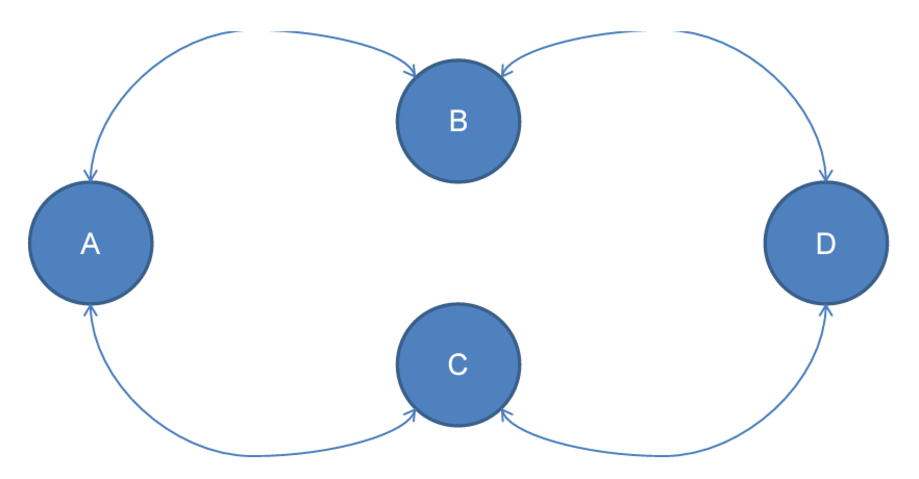
\includegraphics[width=0.5\textheight]{img/contact_example_topology.pdf}
%     \caption{4つのノードからなるDTNの例}
%     \label{fig:contact_example_topology}
%     \begin{minipage}{\textwidth}
%         \centering
%         \vspace{3mm}
%         参考文献\cite{schedule_aware_bundle_routing}figure3-1をもとに作成. 
%     \end{minipage}
% \end{figure}
\begin{table}[htbp]
    \centering
    \caption{図\ref{fig:contact_example_topology}のトポロジーにおけるContact Planの例(Contactに関する表記)}
    \label{table:contact_example_contactplan}
    \begin{minipage}{\textwidth}
        \raggedright
        \vspace{2mm}
        \fontsize{10.5pt}{12pt}\selectfont
        参考文献\cite{schedule_aware_bundle_routing}figure3-2をもとに作成. 
        Senderは送信元のノードの識別子, Receiverは受信元のノードの識別子, FromはContactの開始時刻, Untilは終了時刻, Rateは転送速度を示す.  
        \vspace{2mm}
    \end{minipage}
    \begin{tabular}{cccccc}
      \hline
      Contact & Sender & Recvr & From & Until & Rate \\
      \hline
      1 & A & B & 1000 & 1100 & 1000 \\
      2 & B & A & 1000 & 1100 & 1000 \\
      3 & B & D & 1100 & 1200 & 1000 \\
      4 & D & B & 1100 & 1200 & 1000 \\
      5 & A & C & 1100 & 1200 & 1000 \\
      6 & C & A & 1100 & 1200 & 1000 \\
      7 & A & B & 1300 & 1400 & 1000 \\
      8 & B & A & 1300 & 1400 & 1000 \\
      9 & B & D & 1400 & 1500 & 1000 \\
      10 & D & B & 1400 & 1500 & 1000 \\
      11 & C & D & 1500 & 1600 & 1000 \\
      12 & D & D & 1500 & 1600 & 1000 \\
      \hline
    \end{tabular}
\end{table}
\begin{table}[htbp]
    \centering
    \caption{図\ref{fig:contact_example_topology}のトポロジーにおけるContact Planの例(Rangeに関する表記)}
    \label{table:contact_example_contactrange}
    \begin{minipage}{\textwidth}
        \centering
        \vspace{2mm}
        \fontsize{10.5pt}{12pt}\selectfont
        参考文献\cite{schedule_aware_bundle_routing}figure3-3をもとに作成.  
        \vspace{2mm}
    \end{minipage}
    \begin{tabular}{ccccc}
        \hline
        Sender & Recvr & From & Until & Range (light seconds) \\
        \hline
        A & B & 1000 & 1100 & 1 \\
        A & C & 1100 & 1200 & 30 \\
        B & D & 1400 & 1500 & 120 \\
        C & D & 1500 & 1600 & 90 \\
        \hline
    \end{tabular}
  \end{table}

\section{転送可能な経路の計算}
\label{section:経路決定}

\ref{section:運用計画の決定}節で決定されたContact Planは, 
衛星どうしのContactを記載したものであり, 実際のDTNの運用においては
Contact Planに基づいて転送可能な経路を計算する必要がある.  
ノードAからノードDに向けたBundleを配送する場合, 
表\ref{table:contact_example_contactplan}
及び表\ref{table:contact_example_contactrange}からなるContact Planに対し, 
\ref{section:宇宙インターネットにおけるルーティングのアルゴリズム}項で述べるアルゴリズムを用いることにより
図\ref{fig:contact_example_contactgraph}のようなContact Graphを得る.  
ただしContact Graphにおける頂点はDTNにおける各ノードではなく単一のContactであるため, 
Contact GraphはDTNのトポロジーを示すものではなく, データ転送が可能な経路を計算するためのグラフである.  

% \begin{figure}[tbh]
%     \centering
%     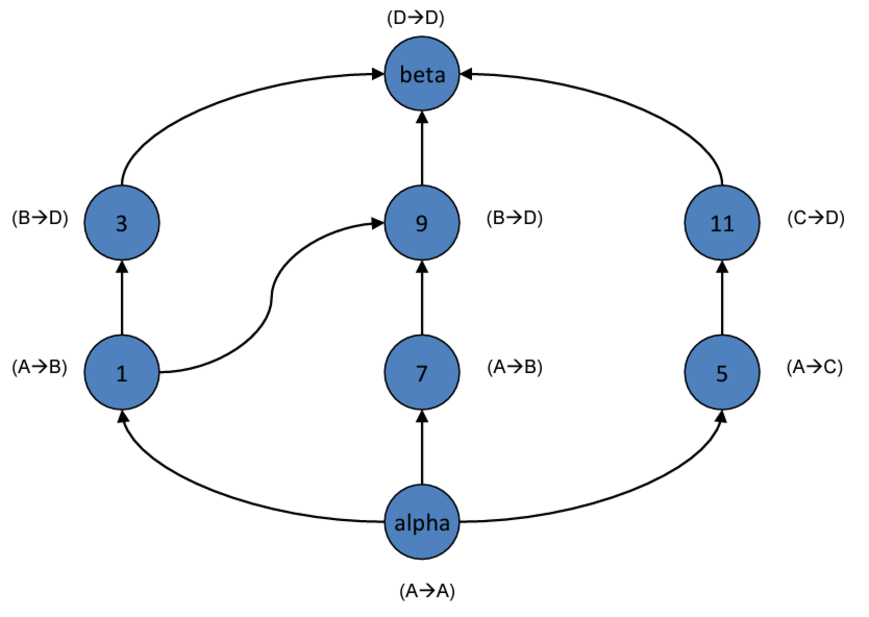
\includegraphics[width=0.5\textheight]{img/contact_example_contactgraph.pdf}
%     \caption{表\ref{table:contact_example_contactplan}及び
%     表\ref{table:contact_example_contactrange}のContact Planから計算されるContact Graphの例}
%     \label{fig:contact_example_contactgraph}
%     \begin{minipage}{\textwidth}
%         \centering
%         \vspace{3mm}
%         参考文献\cite{schedule_aware_bundle_routing}figure3-4をもとに作成.  
%     \end{minipage}
% \end{figure}
% \label{chap:related_works}


\subsection{初期のCGRにおけるルーティングのアルゴリズム}
\label{section:宇宙インターネットにおけるルーティングのアルゴリズム}    
CGRでは図\ref{fig:contact_example_contactgraph}に対してアルゴリズムによる
計算を行うことで最適な転送経路を決定している.  
CGRは\cite{Burleigh2008}において, 基本的なパラメータとContact Graphの利用や, 
これらを用いた転送先の近接ノードの決定などの基本的な概念が提案された.  
しかしこの提案ではルーティングアルゴリズムについては, 静的な経路計算に関する
アルゴリズムは規定されず, ルーティングループ防止の必要性, デフォルトルートを用いた動的
ルーティングの想定などに触れられるのみにとどまった.  

\subsection{CGR-EF}
\label{section:CGR-EF}
Burleighは2010年に\cite{burleigh-dtnrg-cgr-01}において, 
earliest forfeit time, すなわちエンドツーエンドの転送が
可能なパスにおける, そのパスの最短失効時間に注目し, その時間が短いパスから優先して
利用することで, リンク利用の効率化を図るCGR-EFを提案した.  CGR-EFは
2009年10月から11月にかけて行われたディープインパクトネットワーク実験(DINET)
\cite{JPL2009}に用いられ, NASAのジェット推進研究所と宇宙船の間の約300枚の画像転送に成功した.  

\subsection{ECGR}
その後Seguiらは, earliest-forfeit-timeではなくearliest-arrival-time, すなわち
エンドツーエンドの最短到達遅延を指標とするECGRを提案した\cite{6134460}.  
ECGRはearliest-arrival-timeを指標とすることでより計算コストの小さい
ダイクストラアルゴリズムを用いるた経路計算を可能にしており, 
またルーティングループが発生しない, 経路が時間とともに単調に収束することもメリットである.  
これ以後, CGRにおけるアルゴリズムとしては基本的にダイクストラが用いられている.  

\section{最適な経路の決定とBundleの転送}
\label{section:Bundleの転送}

\ref{section:経路決定}節で転送が可能な経路が計算されると, 
これらの計算された経路から最適と考えられる経路が決定され実際にBundleが転送される.  
転送可能な経路が複数存在する場合, \cite{schedule_aware_bundle_routing}では
最適な経路の決定には以下の3点が検証される.  

\begin{itemize}
    \item Earliest transmission opportunity(ETO)
    \item Effective volume limit
    \item Projected arrival time
\end{itemize}

Earliest transmission opportunity (ETO) は, 転送したいBundle(B-object)がネクストホップとなる
隣接ノード(N-next)に転送される最初の時間である.  
現在この転送したいBundleが保持されているノード(N-current)において, 
B-otherが既にキューイングに入っており, B-Xと比較して優先的に転送が行われる場合, 
B-otherがN-currentに存在しない場合と比較してB-objectの
Earliest transmission opportunity (ETO) は遅くなる.  
候補となる経路によって, B-objectのETOは異なるため, 最適な経路の決定の際には考慮される.  

Projected arrival time(PAT)は, B-objectの宛先ノード(N-dest)にB-objectが到着すると予想される時間であり, 
B-objectのTime-to-live(TTL)がこれよりも小さい場合, B-objectは破棄される.  
B-objectのTime-to-live(TTL)がこれよりも大きい場合, 転送可能な経路のうち
最もPATが小さい経路が最適な経路として決定される.  

Effective volume limit(EVL)は選定された経路において, 転送が可能なBundleのサイズの最大値
を示す値であり, この値がB-objectの値よりも小さい場合, B-objectはフラグメンテーションされる.  



\section{Contact Planの定期的・継続的な配布}
\label{section:Contact Planの定期的・継続的な配布}

上記\ref{section:運用計画の決定}節, \ref{section:経路決定}節, \ref{section:Bundleの転送}節
を順に実施することでDTNにおけるCGRが運用されることが想定され, 
これらの手法についての研究がなされている.  
しかし実際の運用においてDTNの各ノードで経路の計算, 決定を行うには, 
さらに\ref{section:運用計画の決定}節で決定されたContact Planを, 
マスターノードからDTNの各ノードに配布する必要がある.  
さらに配布するContact Planは有限時間のContactしか記述しておらず, 
運用時は1度配布するだけでなく定期的・継続的な配布が必要となる.  
Fraireらはノードが保持するDTNのノードの数の増加に対して
Contact Planのサイズが指数関数的に増加することを指摘し, 
そのサイズを減少させる手法の研究を行なった\cite{FRAIRE2018}.  
しかしどのようなサイズのContact Planであっても更新は必要であるが, 
現在その手法に関する標準化はなされていない.  

\section{Contact Planの臨時更新}
\label{section:ContactPlanの臨時更新}
\ref{section:運用計画の決定}節の通り, Contact Planは運用計画の策定時に決定される.  
しかし実際のDTNの運用においては, Contact Planで予定された計画とは異なる場合が存在する.  
Bezirgiannidisらは, 予定外の事象によりContactが失敗する可能性について
指摘し, その情報を他のノードに拡散しContact Planをアップデートすることを提案し, 
Contact Plan Update Protocol(CPUP)を実装した\cite{Bezirgiannidis2013}.  
CPUPを実装したケースにおいては, そうではないケースと比較して
DTNの各ノードが最新のトポロジーを認識できるため, Bundleをより正しい経路に
よって配送することが可能になり, 配送遅延がCPUPが実装されていないケースよりも
低下した. これにより, 想定されていたContactに失敗した場合に, 
その情報をDTNの他のノードに拡散しContact Planを更新することで
配送遅延を低下させることが可能であることが示された. 
以後, 本論文ではこの情報拡散とContact Planの更新をContact Planの臨時更新と呼ぶ. 

\section{Contact Planの臨時更新の課題}
\label{section:ContactPlanの臨時更新の課題}
\ref{section:ContactPlanの臨時更新}節で述べたように, Contact Planの臨時更新は
配送遅延の増加を防ぎネットワークとしての品質を向上することに寄与する. 
しかし実際にContactが失敗した場合, DTNの各ノードにその情報の拡散が完了する時間は, 
拡散を開始するノードからCGRによってその情報を格納したBundleが到達する時間によって決まる.  
そのため天体間にまたがるDTNを運用しており, それらの全てノードに通知を行うことを想定した場合, 
\ref{section:大きな遅延のある通信環境}節で述べた天体間の大きな遅延と, 
さらにその天体内でのContact Planに応じた時間分, 障害情報の拡散の完了までには大きな時間を要する.  
Bezirgiannidisらの研究で行われたCPUPの実装でも, DTNの全てのノードに対して
臨時更新を行うことを前提としているが, 情報が天体間遅延を超えて拡散した時点で, 
既に当該Contactは古くて使われない経路になっている場合も存在するため, 
運用するDTNのContact Planによっても, 全てのノードか
天体内のノードのみかなど臨時更新の対象の対象を選定する必要がある.  
またContactの障害情報を拡散することは, その通知のために貴重な天体間のリンクに余計な
Bundleが発生する. またその情報を受け取ったノードでの再計算を伴い, 
さらにトラフィックが一部のノードに集中することにもなり得るため, 
DTNの運用におけるこれらの影響についても考慮する必要がある. 
そのためContact Planの臨時更新の対象は,
そのノードに拡散することによるBundleの配送能力の向上度合いとネットワークへの負荷の変化
に応じて対象を工夫する必要性が存在する.  